\documentclass{standalone}
\usepackage{tikz}
\usetikzlibrary{patterns, positioning}


\begin{document}
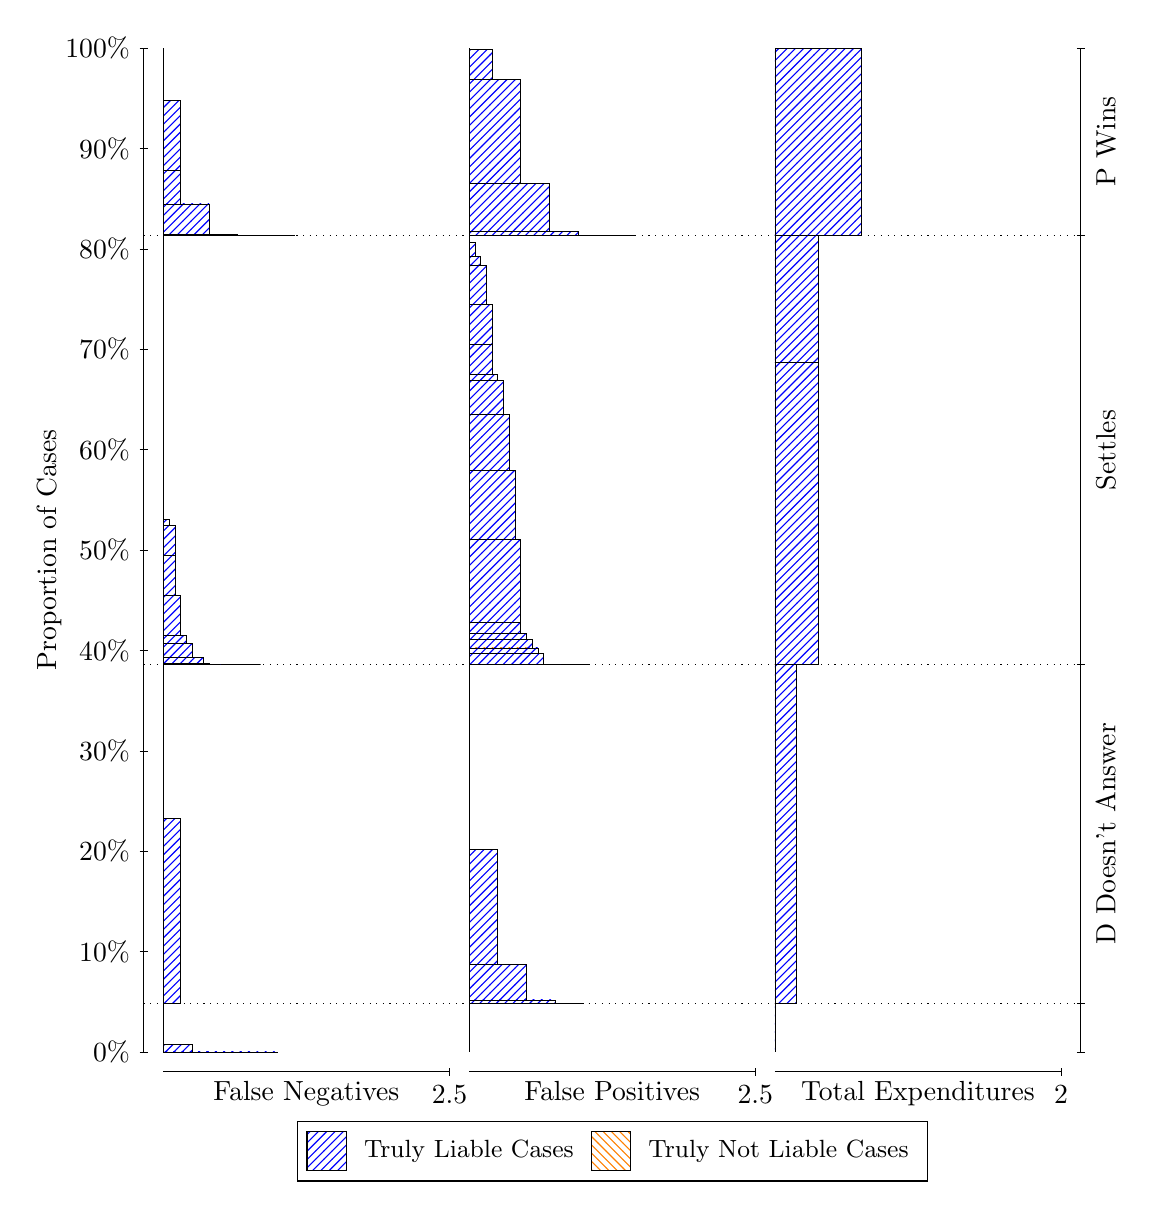
\begin{tikzpicture}
\draw[black, very thin] (1.5,1.75) -- (1.5,14.5);
\node[rotate=90, text=black, anchor=center] at (0.3, 8.125) {Proportion of Cases};
\draw[black, very thin] (1.45,1.75) -- (1.55,1.75);
\node[text=black, anchor=east] at (1.45, 1.75) {0\%};
\draw[black, very thin] (1.45,3.025) -- (1.55,3.025);
\node[text=black, anchor=east] at (1.45, 3.025) {10\%};
\draw[black, very thin] (1.45,4.3) -- (1.55,4.3);
\node[text=black, anchor=east] at (1.45, 4.3) {20\%};
\draw[black, very thin] (1.45,5.575) -- (1.55,5.575);
\node[text=black, anchor=east] at (1.45, 5.575) {30\%};
\draw[black, very thin] (1.45,6.85) -- (1.55,6.85);
\node[text=black, anchor=east] at (1.45, 6.85) {40\%};
\draw[black, very thin] (1.45,8.125) -- (1.55,8.125);
\node[text=black, anchor=east] at (1.45, 8.125) {50\%};
\draw[black, very thin] (1.45,9.4) -- (1.55,9.4);
\node[text=black, anchor=east] at (1.45, 9.4) {60\%};
\draw[black, very thin] (1.45,10.675) -- (1.55,10.675);
\node[text=black, anchor=east] at (1.45, 10.675) {70\%};
\draw[black, very thin] (1.45,11.95) -- (1.55,11.95);
\node[text=black, anchor=east] at (1.45, 11.95) {80\%};
\draw[black, very thin] (1.45,13.225) -- (1.55,13.225);
\node[text=black, anchor=east] at (1.45, 13.225) {90\%};
\draw[black, very thin] (1.45,14.5) -- (1.55,14.5);
\node[text=black, anchor=east] at (1.45, 14.5) {100\%};

\draw[black, very thin] (13.4,1.75) -- (13.4,14.5);
\draw[black, very thin] (13.35,1.75) -- (13.45,1.75);
\node[anchor=west] at (13.35, 1.75) {};
\draw[black, very thin] (13.35,2.3686) -- (13.45,2.3686);
\node[anchor=west] at (13.35, 2.3686) {};
\draw[black, very thin] (13.35,6.6718) -- (13.45,6.6718);
\node[anchor=west] at (13.35, 6.6718) {};
\draw[black, very thin] (13.35,12.119) -- (13.45,12.119);
\node[anchor=west] at (13.35, 12.119) {};
\draw[black, very thin] (13.35,14.5) -- (13.45,14.5);
\node[anchor=west] at (13.35, 14.5) {};

\draw[black, very thin, pattern color=blue, pattern=north east lines] (1.75,1.75) rectangle (3.2033,1.75);
\draw[black, very thin, pattern color=blue, pattern=north east lines] (1.75,1.75) rectangle (2.84,1.75);
\draw[black, very thin, pattern color=blue, pattern=north east lines] (1.75,1.75) rectangle (2.4767,1.7509);
\draw[black, very thin, pattern color=blue, pattern=north east lines] (1.75,1.7509) rectangle (2.1133,1.8513);
\draw[black, very thin, pattern color=orange, pattern=north west lines] (1.75,1.8513) rectangle (1.75,1.8513);
\draw[black, very thin, pattern color=blue, pattern=north east lines] (1.75,1.8513) rectangle (1.75,2.3686);
\draw[black, very thin, pattern color=blue, pattern=north east lines] (1.75,2.3686) rectangle (1.968,4.714);
\draw[black, very thin, pattern color=orange, pattern=north west lines] (1.75,4.714) rectangle (1.75,4.714);
\draw[black, very thin, pattern color=blue, pattern=north east lines] (1.75,4.714) rectangle (1.75,6.6718);
\draw[black, very thin, pattern color=blue, pattern=north east lines] (1.75,6.6718) rectangle (2.9853,6.6718);
\draw[black, very thin, pattern color=blue, pattern=north east lines] (1.75,6.6718) rectangle (2.84,6.6718);
\draw[black, very thin, pattern color=blue, pattern=north east lines] (1.75,6.6718) rectangle (2.6947,6.6718);
\draw[black, very thin, pattern color=blue, pattern=north east lines] (1.75,6.6718) rectangle (2.622,6.6719);
\draw[black, very thin, pattern color=blue, pattern=north east lines] (1.75,6.6719) rectangle (2.5493,6.6719);
\draw[black, very thin, pattern color=blue, pattern=north east lines] (1.75,6.6719) rectangle (2.4767,6.6719);
\draw[black, very thin, pattern color=blue, pattern=north east lines] (1.75,6.6719) rectangle (2.404,6.6721);
\draw[black, very thin, pattern color=blue, pattern=north east lines] (1.75,6.6721) rectangle (2.3313,6.6883);
\draw[black, very thin, pattern color=blue, pattern=north east lines] (1.75,6.6883) rectangle (2.2587,6.7589);
\draw[black, very thin, pattern color=blue, pattern=north east lines] (1.75,6.7589) rectangle (2.186,6.7592);
\draw[black, very thin, pattern color=blue, pattern=north east lines] (1.75,6.7592) rectangle (2.1133,6.9405);
\draw[black, very thin, pattern color=blue, pattern=north east lines] (1.75,6.9405) rectangle (2.0407,7.0448);
\draw[black, very thin, pattern color=blue, pattern=north east lines] (1.75,7.0448) rectangle (1.968,7.5456);
\draw[black, very thin, pattern color=blue, pattern=north east lines] (1.75,7.5456) rectangle (1.8953,8.0547);
\draw[black, very thin, pattern color=blue, pattern=north east lines] (1.75,8.0547) rectangle (1.8953,8.4341);
\draw[black, very thin, pattern color=blue, pattern=north east lines] (1.75,8.4341) rectangle (1.8227,8.5096);
\draw[black, very thin, pattern color=orange, pattern=north west lines] (1.75,8.5096) rectangle (1.75,8.5096);
\draw[black, very thin, pattern color=blue, pattern=north east lines] (1.75,8.5096) rectangle (1.75,12.119);
\draw[black, very thin, pattern color=blue, pattern=north east lines] (1.75,12.119) rectangle (3.4213,12.119);
\draw[black, very thin, pattern color=blue, pattern=north east lines] (1.75,12.119) rectangle (3.058,12.119);
\draw[black, very thin, pattern color=blue, pattern=north east lines] (1.75,12.119) rectangle (2.6947,12.138);
\draw[black, very thin, pattern color=blue, pattern=north east lines] (1.75,12.138) rectangle (2.3313,12.522);
\draw[black, very thin, pattern color=blue, pattern=north east lines] (1.75,12.522) rectangle (1.968,12.944);
\draw[black, very thin, pattern color=blue, pattern=north east lines] (1.75,12.944) rectangle (1.968,13.836);
\draw[black, very thin, pattern color=orange, pattern=north west lines] (1.75,13.836) rectangle (1.75,13.836);
\draw[black, very thin, pattern color=blue, pattern=north east lines] (1.75,13.836) rectangle (1.75,14.5);
\draw[black, very thin, pattern color=orange, pattern=north west lines] (5.6333,1.75) rectangle (5.6333,1.75);
\draw[black, very thin, pattern color=blue, pattern=north east lines] (5.6333,1.75) rectangle (5.6333,2.3686);
\draw[black, very thin, pattern color=orange, pattern=north west lines] (5.6333,2.3686) rectangle (7.0867,2.3686);
\draw[black, very thin, pattern color=blue, pattern=north east lines] (5.6333,2.3686) rectangle (7.0867,2.3687);
\draw[black, very thin, pattern color=blue, pattern=north east lines] (5.6333,2.3687) rectangle (6.7233,2.4129);
\draw[black, very thin, pattern color=blue, pattern=north east lines] (5.6333,2.4129) rectangle (6.36,2.8657);
\draw[black, very thin, pattern color=blue, pattern=north east lines] (5.6333,2.8657) rectangle (5.9967,4.3263);
\draw[black, very thin, pattern color=blue, pattern=north east lines] (5.6333,4.3263) rectangle (5.6333,6.6718);
\draw[black, very thin, pattern color=orange, pattern=north west lines] (5.6333,6.6718) rectangle (7.1593,6.6718);
\draw[black, very thin, pattern color=blue, pattern=north east lines] (5.6333,6.6718) rectangle (7.1593,6.6718);
\draw[black, very thin, pattern color=orange, pattern=north west lines] (5.6333,6.6718) rectangle (7.014,6.6718);
\draw[black, very thin, pattern color=blue, pattern=north east lines] (5.6333,6.6718) rectangle (7.014,6.6718);
\draw[black, very thin, pattern color=orange, pattern=north west lines] (5.6333,6.6718) rectangle (6.8687,6.6718);
\draw[black, very thin, pattern color=blue, pattern=north east lines] (5.6333,6.6718) rectangle (6.8687,6.6719);
\draw[black, very thin, pattern color=blue, pattern=north east lines] (5.6333,6.6719) rectangle (6.796,6.6719);
\draw[black, very thin, pattern color=orange, pattern=north west lines] (5.6333,6.6719) rectangle (6.7233,6.6719);
\draw[black, very thin, pattern color=blue, pattern=north east lines] (5.6333,6.6719) rectangle (6.7233,6.6725);
\draw[black, very thin, pattern color=blue, pattern=north east lines] (5.6333,6.6725) rectangle (6.6507,6.673);
\draw[black, very thin, pattern color=orange, pattern=north west lines] (5.6333,6.673) rectangle (6.578,6.673);
\draw[black, very thin, pattern color=blue, pattern=north east lines] (5.6333,6.673) rectangle (6.578,6.816);
\draw[black, very thin, pattern color=blue, pattern=north east lines] (5.6333,6.816) rectangle (6.5053,6.8827);
\draw[black, very thin, pattern color=orange, pattern=north west lines] (5.6333,6.8827) rectangle (6.4327,6.8827);
\draw[black, very thin, pattern color=blue, pattern=north east lines] (5.6333,6.8827) rectangle (6.4327,6.9927);
\draw[black, very thin, pattern color=blue, pattern=north east lines] (5.6333,6.9927) rectangle (6.36,7.0696);
\draw[black, very thin, pattern color=blue, pattern=north east lines] (5.6333,7.0696) rectangle (6.2873,7.2056);
\draw[black, very thin, pattern color=orange, pattern=north west lines] (5.6333,7.2056) rectangle (6.2873,7.2056);
\draw[black, very thin, pattern color=blue, pattern=north east lines] (5.6333,7.2056) rectangle (6.2873,8.2613);
\draw[black, very thin, pattern color=blue, pattern=north east lines] (5.6333,8.2613) rectangle (6.2147,9.1369);
\draw[black, very thin, pattern color=blue, pattern=north east lines] (5.6333,9.1369) rectangle (6.142,9.8506);
\draw[black, very thin, pattern color=blue, pattern=north east lines] (5.6333,9.8506) rectangle (6.0693,10.281);
\draw[black, very thin, pattern color=blue, pattern=north east lines] (5.6333,10.281) rectangle (5.9967,10.357);
\draw[black, very thin, pattern color=blue, pattern=north east lines] (5.6333,10.357) rectangle (5.924,10.736);
\draw[black, very thin, pattern color=blue, pattern=north east lines] (5.6333,10.736) rectangle (5.924,11.245);
\draw[black, very thin, pattern color=blue, pattern=north east lines] (5.6333,11.245) rectangle (5.8513,11.746);
\draw[black, very thin, pattern color=blue, pattern=north east lines] (5.6333,11.746) rectangle (5.7787,11.851);
\draw[black, very thin, pattern color=blue, pattern=north east lines] (5.6333,11.851) rectangle (5.706,12.032);
\draw[black, very thin, pattern color=blue, pattern=north east lines] (5.6333,12.032) rectangle (5.6333,12.119);
\draw[black, very thin, pattern color=orange, pattern=north west lines] (5.6333,12.119) rectangle (7.7407,12.119);
\draw[black, very thin, pattern color=blue, pattern=north east lines] (5.6333,12.119) rectangle (7.7407,12.119);
\draw[black, very thin, pattern color=orange, pattern=north west lines] (5.6333,12.119) rectangle (7.3773,12.119);
\draw[black, very thin, pattern color=blue, pattern=north east lines] (5.6333,12.119) rectangle (7.3773,12.12);
\draw[black, very thin, pattern color=orange, pattern=north west lines] (5.6333,12.12) rectangle (7.014,12.12);
\draw[black, very thin, pattern color=blue, pattern=north east lines] (5.6333,12.12) rectangle (7.014,12.174);
\draw[black, very thin, pattern color=orange, pattern=north west lines] (5.6333,12.174) rectangle (6.6507,12.174);
\draw[black, very thin, pattern color=blue, pattern=north east lines] (5.6333,12.174) rectangle (6.6507,12.783);
\draw[black, very thin, pattern color=orange, pattern=north west lines] (5.6333,12.783) rectangle (6.2873,12.783);
\draw[black, very thin, pattern color=blue, pattern=north east lines] (5.6333,12.783) rectangle (6.2873,14.097);
\draw[black, very thin, pattern color=blue, pattern=north east lines] (5.6333,14.097) rectangle (5.924,14.481);
\draw[black, very thin, pattern color=blue, pattern=north east lines] (5.6333,14.481) rectangle (5.6333,14.5);
\draw[black, very thin, pattern color=orange, pattern=north west lines] (9.5167,1.75) rectangle (9.5167,1.75);
\draw[black, very thin, pattern color=blue, pattern=north east lines] (9.5167,1.75) rectangle (9.5167,2.3686);
\draw[black, very thin, pattern color=orange, pattern=north west lines] (9.5167,2.3686) rectangle (9.7892,2.3686);
\draw[black, very thin, pattern color=blue, pattern=north east lines] (9.5167,2.3686) rectangle (9.7892,6.6718);
\draw[black, very thin, pattern color=orange, pattern=north west lines] (9.5167,6.6718) rectangle (10.062,6.6718);
\draw[black, very thin, pattern color=blue, pattern=north east lines] (9.5167,6.6718) rectangle (10.062,10.504);
\draw[black, very thin, pattern color=orange, pattern=north west lines] (9.5167,10.504) rectangle (10.062,10.504);
\draw[black, very thin, pattern color=blue, pattern=north east lines] (9.5167,10.504) rectangle (10.062,12.119);
\draw[black, very thin, pattern color=orange, pattern=north west lines] (9.5167,12.119) rectangle (10.607,12.119);
\draw[black, very thin, pattern color=blue, pattern=north east lines] (9.5167,12.119) rectangle (10.607,14.5);
\draw[black, dotted] (1.5,2.3686) -- (13.4,2.3686);
\draw[black, dotted] (1.5,6.6718) -- (13.4,6.6718);
\draw[black, dotted] (1.5,12.119) -- (13.4,12.119);
\draw[black, very thin] (1.75,1.5) -- (5.3833,1.5);
\node[text=black, anchor=north] at (3.5667, 1.5) {False Negatives};
\draw[black, very thin] (5.3833,1.45) -- (5.3833,1.55);
\node[text=black, anchor=north] at (5.3833, 1.45) {2.5};

\draw[black, very thin] (5.6333,1.5) -- (9.2667,1.5);
\node[text=black, anchor=north] at (7.45, 1.5) {False Positives};
\draw[black, very thin] (9.2667,1.45) -- (9.2667,1.55);
\node[text=black, anchor=north] at (9.2667, 1.45) {2.5};

\draw[black, very thin] (9.5167,1.5) -- (13.15,1.5);
\node[text=black, anchor=north] at (11.333, 1.5) {Total Expenditures};
\draw[black, very thin] (13.15,1.45) -- (13.15,1.55);
\node[text=black, anchor=north] at (13.15, 1.45) {2};


\node[text=black, centered, rotate=90] at (13.72, 4.5202) {D Doesn't Answer};
\node[text=black, centered, rotate=90] at (13.72, 9.3955) {Settles};
\node[text=black, centered, rotate=90] at (13.72, 13.31) {P Wins};

\draw (7.449999999999999,1.5) node[draw=none] (baseCoordinate) {};
\begin{scope}[align=center]
        \matrix[scale=0.5, draw=black, below=0.5cm of baseCoordinate, nodes={draw}, column sep=0.1cm]{
            \node[rectangle, draw, minimum width=0.5cm, minimum height=0.5cm, pattern color=blue, pattern=north east lines] {}; &
            \node[draw=none, font=\small, text=black] (B) {Truly Liable Cases}; &
            \node[rectangle, draw, minimum width=0.5cm, minimum height=0.5cm, pattern color=orange, pattern=north west lines] {}; &
            \node[draw=none, font=\small, text=black] (B) {Truly Not Liable Cases}; \\
            };
\end{scope}

\end{tikzpicture}
\end{document}